\documentclass[tikz,border=10pt]{standalone}
\usepackage{amsmath,amssymb}
\usetikzlibrary{positioning, arrows.meta, calc}

\begin{document}
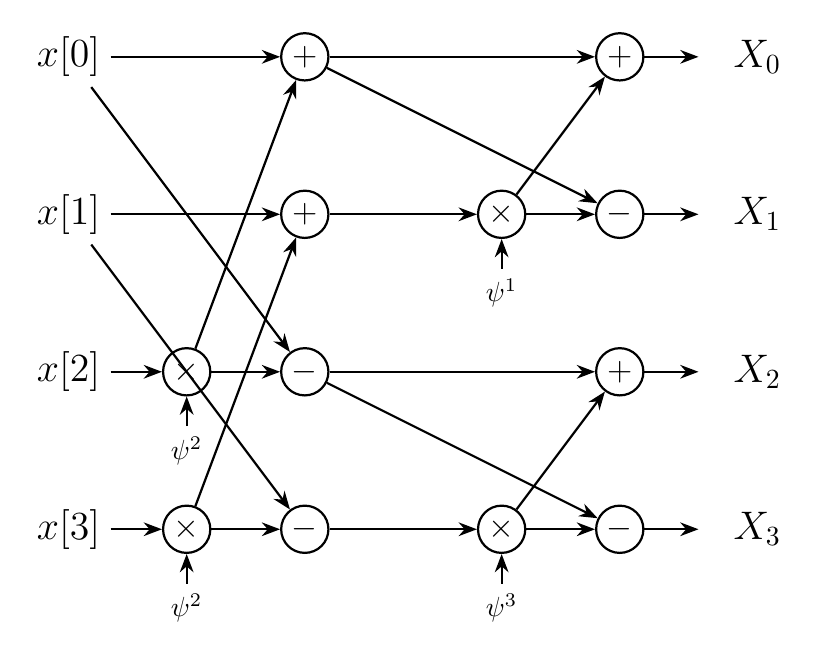
\begin{tikzpicture}[
    >=Stealth, 
    node distance=1.5cm, 
    thick,
    op/.style={circle, draw, minimum size=0.6cm, inner sep=0pt, font=\large},
    input/.style={font=\Large},
    twiddle/.style={font=\normalsize, above, midway}
]

    % --- Coordenadas Verticais das Linhas ---
    % Linhas 0, 1, 2, 3 de cima para baixo
    \coordinate (L0) at (0, 0);
    \coordinate (L1) at (0, -2);
    \coordinate (L2) at (0, -4);
    \coordinate (L3) at (0, -6);

    % --- Entradas (Ordem Natural) ---
    \node[input] (in0) at (L0) {$x[0]$};
    \node[input] (in1) at (L1) {$x[1]$};
    \node[input] (in2) at (L2) {$x[2]$};
    \node[input] (in3) at (L3) {$x[3]$};

    % ==================================================
    % ESTÁGIO 1: Stride 2 (N=4 -> N=2)
    % Combina x[0] com x[2] e x[1] com x[3]
    % Twiddle usado: \psi^2 (pois N=4, N/2=2)
    % ==================================================

    % --- Operadores do Par 1 (Linhas 0 e 2) ---
    \node[op] (plus1_0) at (3, 0) {$+$};
    \node[op] (minus1_2) at (3, -4) {$-$};
    \node[op] (times1_2) at (1.5, -4) {$\times$}; % Multiplicador na linha de baixo
    \node (psi1) at (1.5, -5) {$\psi^2$};        % Fator de rotação

    % Conexões Estágio 1 - Par 1
    \draw[->] (in0) -- (plus1_0);                     % x[0] -> +
    \draw[->] (in0) -- (minus1_2);                    % x[0] -> - (cruzado)
    \draw[->] (in2) -- (times1_2);                    % x[2] -> x
    \draw[->] (psi1) -- (times1_2);                   % fator -> x
    \draw[->] (times1_2) -- (minus1_2);               % x -> -
    \draw[->] (times1_2) -- (plus1_0);                % x -> + (cruzado)

    % --- Operadores do Par 2 (Linhas 1 e 3) ---
    \node[op] (plus1_1) at (3, -2) {$+$};
    \node[op] (minus1_3) at (3, -6) {$-$};
    \node[op] (times1_3) at (1.5, -6) {$\times$};
    \node (psi2) at (1.5, -7) {$\psi^2$};

    % Conexões Estágio 1 - Par 2
    \draw[->] (in1) -- (plus1_1);
    \draw[->] (in1) -- (minus1_3);
    \draw[->] (in3) -- (times1_3);
    \draw[->] (psi2) -- (times1_3);
    \draw[->] (times1_3) -- (minus1_3);
    \draw[->] (times1_3) -- (plus1_1);

    % ==================================================
    % ESTÁGIO 2: Stride 1 (N=2 -> N=1)
    % Combina vizinhos. 
    % Twiddles: \psi^1 (topo) e \psi^3 (fundo)
    % ==================================================

    % --- Operadores do Topo (Resultados anteriores de 0 e 1) ---
    \node[op] (plus2_0) at (7, 0) {$+$};
    \node[op] (minus2_1) at (7, -2) {$-$};
    \node[op] (times2_1) at (5.5, -2) {$\times$};
    \node (psi3) at (5.5, -3) {$\psi^1$}; 

    % Conexões Topo
    \draw[->] (plus1_0) -- (plus2_0);       % 0 -> 0
    \draw[->] (plus1_0) -- (minus2_1);      % 0 -> 1
    \draw[->] (plus1_1) -- (times2_1);      % 1 -> x
    \draw[->] (psi3) -- (times2_1);
    \draw[->] (times2_1) -- (minus2_1);     % 1 -> 1
    \draw[->] (times2_1) -- (plus2_0);      % 1 -> 0

    % --- Operadores do Fundo (Resultados anteriores de 2 e 3) ---
    \node[op] (plus2_2) at (7, -4) {$+$};
    \node[op] (minus2_3) at (7, -6) {$-$};
    \node[op] (times2_3) at (5.5, -6) {$\times$};
    \node (psi4) at (5.5, -7) {$\psi^3$};

    % Conexões Fundo
    \draw[->] (minus1_2) -- (plus2_2);      % 2 -> 2
    \draw[->] (minus1_2) -- (minus2_3);     % 2 -> 3
    \draw[->] (minus1_3) -- (times2_3);     % 3 -> x
    \draw[->] (psi4) -- (times2_3);
    \draw[->] (times2_3) -- (minus2_3);     % 3 -> 3
    \draw[->] (times2_3) -- (plus2_2);      % 3 -> 2

    % --- Saídas (Bit-Reversed se fosse DIF puro, mas aqui são os ramos do CRT) ---
    \node[right=1cm of plus2_0]  {\Large $X_0$};
    \node[right=1cm of minus2_1] {\Large $X_1$};
    \node[right=1cm of plus2_2]  {\Large $X_2$};
    \node[right=1cm of minus2_3] {\Large $X_3$};

    \draw[->] (plus2_0) -- +(1,0);
    \draw[->] (minus2_1) -- +(1,0);
    \draw[->] (plus2_2) -- +(1,0);
    \draw[->] (minus2_3) -- +(1,0);

\end{tikzpicture}
\end{document}